\chapter{构建阀盖立三维模型}

{\bfseries 学习目标}
\begin{itemize}
\item 学习利用xline命令的角度选项绘制图形
\item 学习利用arc命令绘图形
\item 学习利用union命令构建三维模型
\item 学习利用创建布局向导创建布局
\item 掌握基本几何体的三视图表达
\item 学习利用viewbase命令生成基本视图
\end{itemize}

{\bfseries 任务要求}
\begin{itemize}
\item 根据图\ref{fig:tiaoyafafagai}所示的杯零件图,用拉伸法建立调压阀阀盖零件的三维模型
\item 利用阀盖三维模型生成基本三视图
\end{itemize}

\noindent
\begin{figure}[htbp]
\centering
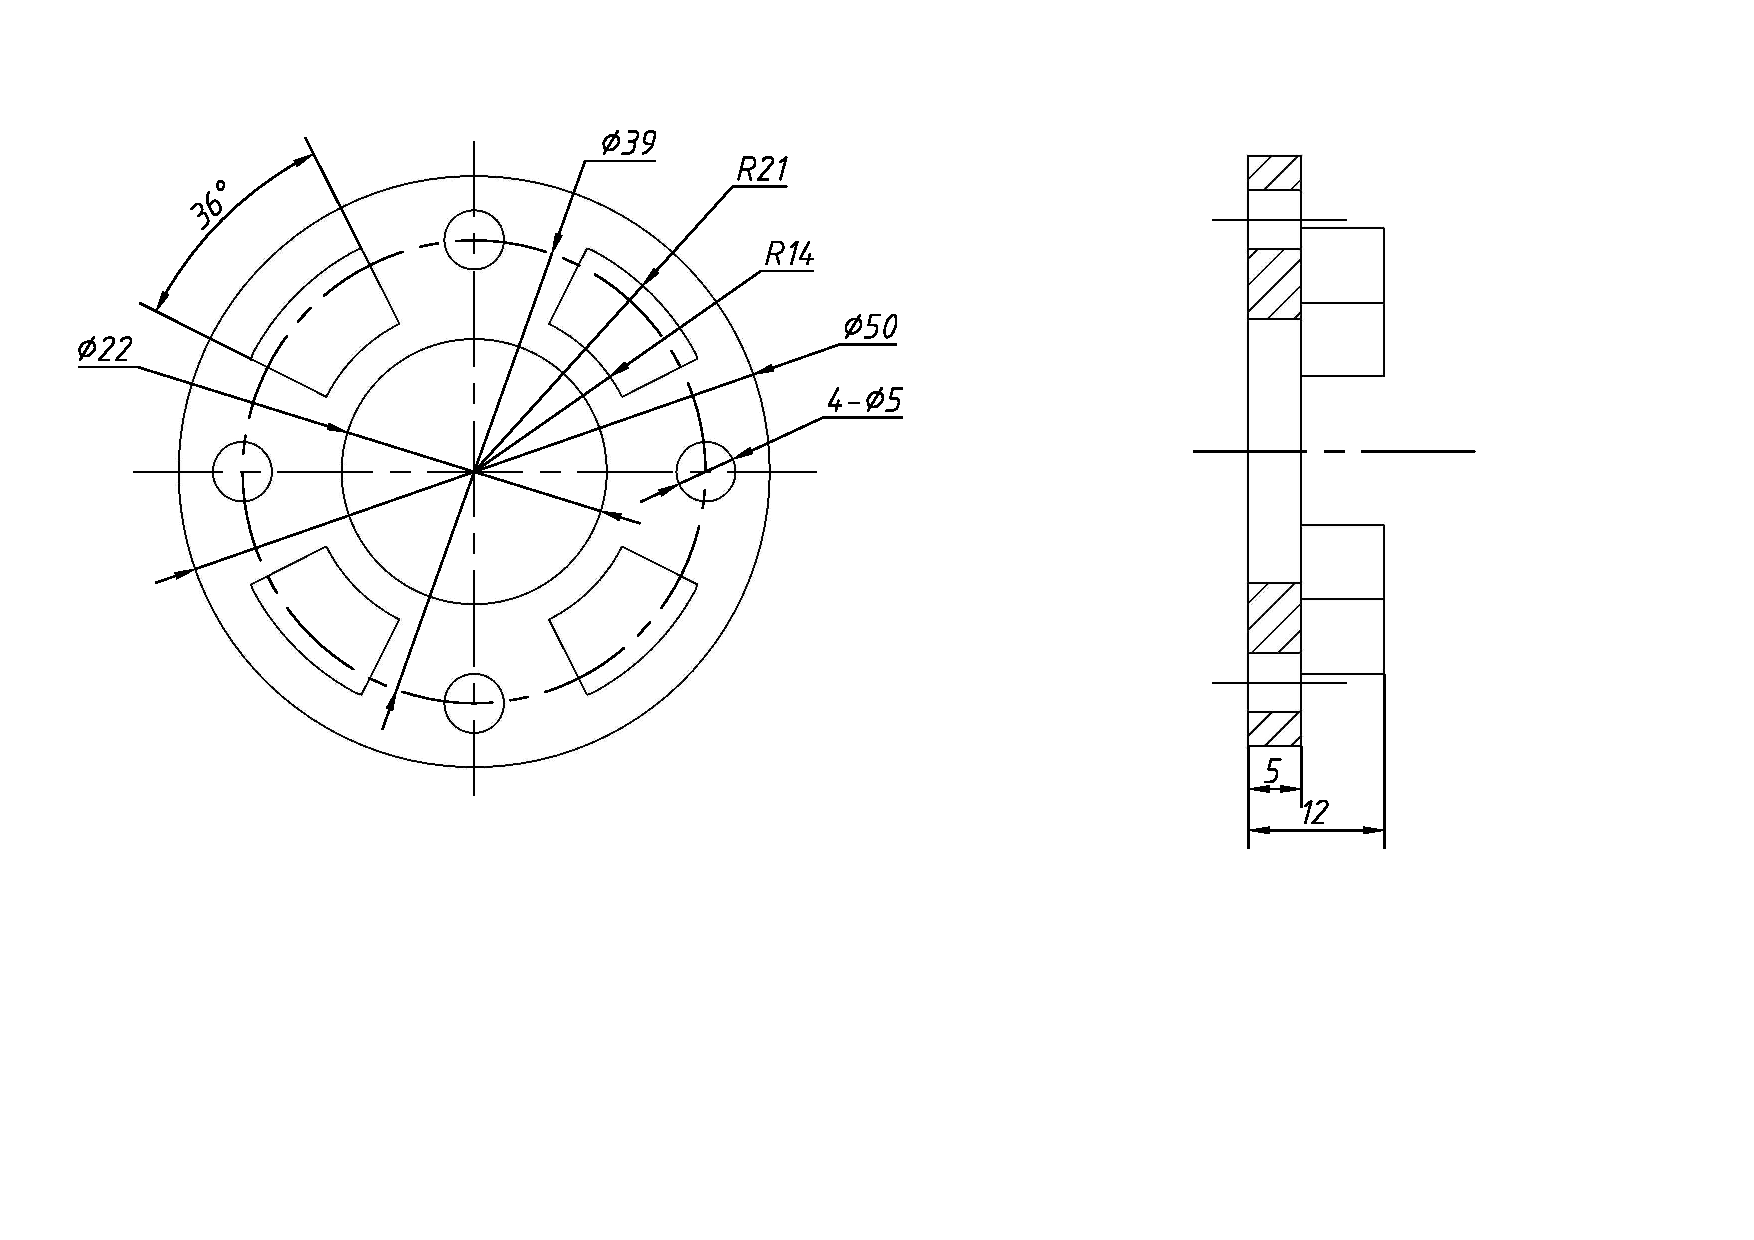
\includegraphics[scale=0.6]{tiaoyafafagai.pdf}
\caption{阀盖零件图}\label{fig:tiaoyafafagai}
\end{figure}
\clearpage

根据表面形状的不同可以将基本几何体分为平面立体和曲面立体。如果立体表面均由平面构成,则称为平面立体,如长方体、正方体、棱柱、棱锥、棱台等。如果立体表面由平面和曲面共同构成或全部由曲面构成,则称为曲面立体,如圆柱、圆球、圆环等。
\subsection{平面立体}
在平面立体中,平面立体的表面是由若干个平面多边形构成的,多边形的边是平面立体的轮廓线,是平面立体两个平面的交线,当轮廓的投影可见时,用粗实线表示;不可见时,用虚线表示;当实线与虚线重合时,应当用粗实线表示。
\subsubsection{棱柱体}
棱柱体由顶面、底面及若干个侧棱面构成。棱柱体的各个侧棱相互平行,顶面和底面相互平行。如果棱柱的侧棱与顶面和底面垂直则称为直棱柱,否则称为斜棱柱。当直棱柱的顶面和底面为正多边形时则称为正棱柱。
\begin{figure}[htbp]
\centering
\subfloat[]{\label{fig:cube}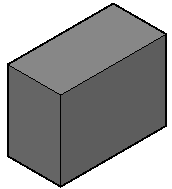
\includegraphics[scale=0.9]{cube.png}}\hspace{30pt}
\subfloat[]{\label{fig:cubethreeview}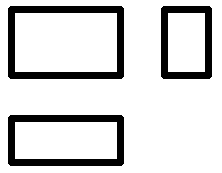
\includegraphics[scale=1]{cubethreeview.png}}
\caption{长方体的投影}
\end{figure}

图\ref{fig:cubethreeview}所示的长方体,其顶面与底面的水平投影重合并反映衬形,为一长方形,其它棱面的水平投影积聚为长方形的四条边;前面与后面的正投影重合并反映实形,顶面、底面和两个侧面积聚为长方形的四条件边;左面和右面的侧面投影重合并反映实形,顶面、底面、前面和后面积聚为长方形的四条件边。长方体的三视图投影如图\ref{fig:cube}所示。

图\ref{fig:sannenzhu}所示的正三棱柱,其顶面与底面的水平面投影重合并反映实形,为一正三角形。三个棱面在水平投影面积聚为三角形的三条边。三棱柱的三视图投影如图\ref{fig:sannenzhuthreeview}所示。
\begin{figure}[htbp]
\centering
\subfloat[]{\label{fig:sannenzhu}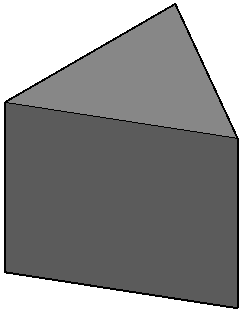
\includegraphics[scale=0.6]{sannenzhu.png}}\hspace{30pt}
\subfloat[]{\label{fig:sannenzhuthreeview}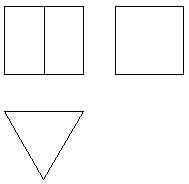
\includegraphics[scale=1]{sannenzhuthreeview.png}}
\caption{正三棱柱的投影}
\end{figure}

图\ref{fig:sixnenzhu}所示的正六棱柱,其顶面与底面的水平面投影重合并反映实形,为一正六边形。六个棱面在水平投影面积聚为六边形的六条边。正六棱柱的三视较长投影如图\ref{fig:sixnenthreeview}所示。
\begin{figure}[htbp]
\centering
\subfloat[]{\label{fig:sixnenzhu}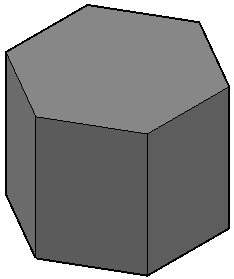
\includegraphics[scale=0.7]{sixnenzhu.png}}\hspace{30pt}
\subfloat[]{\label{fig:sixnenthreeview}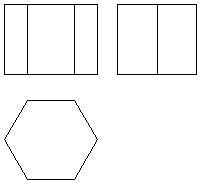
\includegraphics[scale=1]{sixnenthreeview.png}}
\caption{正六棱柱的投影}
\end{figure}

由此可见棱柱体的投影特点是:一面投影反映底面实形,其余两面投影则为矩形或复合矩形。
\subsubsection{棱锥体}
棱锥体是由一个多边形底面和若干个共顶点的三角形棱面构成的。从棱锥体顶点到底面的垂直距离称为棱锥体的高。如果棱锥体的底面为正多边形,锥顶的投影位于多边形的中心,各棱面是等腰三角形,则该棱锥体称为正棱锥。正四棱锥的三面投影如图\ref{fig:fournenzhuithreeview}所示。

\begin{figure}[htbp]
\centering
\subfloat[]{\label{fig:fournengzhui}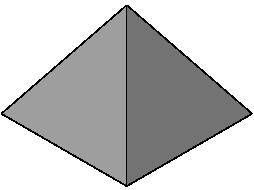
\includegraphics[scale=0.9]{fournengzhui.png}}\hspace{30pt}
\subfloat[]{\label{fig:fournenzhuithreeview}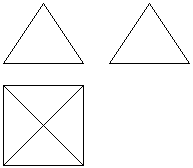
\includegraphics[scale=1]{fournenzhuithreeview.png}}
\caption{正四棱锥的投影}
\end{figure}

图\ref{fig:fournengzhui}所示的正四棱锥的底面与水平投影面平行,其投影反映实形,为正方形;底面在其它投影面积聚为一条直线;棱面的三面投影则为类似的三角形。

由此可见,棱锥体的投影特点是:一投影面为由三角形构成的复合多边形,其两投影为三角形或复合三角形。
\subsubsection{棱台体}
棱台体是由棱锥体被切掉顶部后所构成的一种形体。棱台体的投影特点是:一面投影为由梯形构成的内外相似复合多边形,其余两面投影则为梯形或复合梯形。图\ref{fig:fivenentai} 所示为五棱台的投影。
\begin{figure}[htbp]
\centering
\subfloat[]{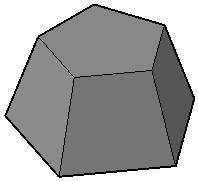
\includegraphics[scale=0.9]{fivenentai.png}}\hspace{30pt}
\subfloat[]{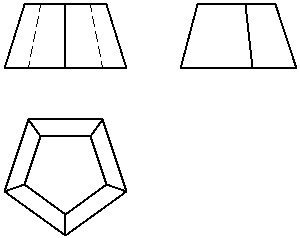
\includegraphics[scale=1]{fivenentaithreeview.png}}
\caption{五棱台的投影}\label{fig:fivenentai}
\end{figure}

\endinput
\subsection{曲面立体}
曲面体是由面或曲面和平面共同构成的立体,其中最常见的是回转曲面。回转体曲面是由一母线绕一空间轴线作旋转运动而形成的光滑曲面。母线在在回转曲面上任意位置称作素线,母线上任意一点的旋转轨迹都是一个圆,该圆称为纬圆。图\ref{fig:huizhuangti}所示为回转体的形成和术语。
\begin{figure}[htbp]
\centering
\subfloat[]{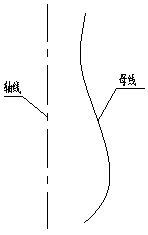
\includegraphics[scale=0.5]{huizhuangti.png}}\hspace{30pt}
\subfloat[]{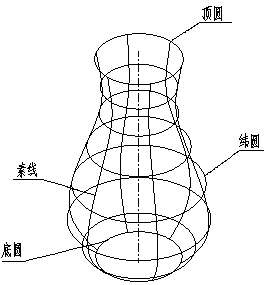
\includegraphics[scale=0.5]{rotatetree.png}}
\caption{回转体的形成及术语}\label{fig:huizhuangti}
\end{figure}

画回转体的投影图时,首先画出回转轴线,然后画出反映实形的投影,最后画其余两个投影。回转曲面向某一投影面投影时,轮廓素线是回转曲面在该投影面上可见和不可见面的分界线的投影,在分界线之前的回转曲面为可见,反之则不可见。画图时,凡不属于该投影面的轮廓素线,一律不画出。
\subsubsection{圆柱体}
圆柱体是由圆柱面、顶面、底面所构成的。圆柱体可以看作一条与轴线平行的母线绕轴线旋转而成的。图所示圆柱体的轴线垂直于水平投影面,其水平投影为圆;其正投影和侧投影均为矩形。
\begin{figure}[htbp]
\centering
\subfloat[]{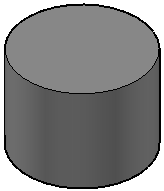
\includegraphics[scale=0.9]{yuanzhuti.png}}\hspace{30pt}
\subfloat[]{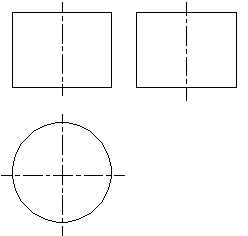
\includegraphics[scale=0.7]{yuanzhutithreeview.png}}
\caption{圆柱体的投影}\label{fig:yuanzhuti}
\end{figure}
\subsubsection{圆锥体}
图\ref{fig:yuanzhuiti} 所示的圆锥体底面与水平投影面平行,其投影为一圆,反映实形,在其余两个投影面上积聚为一条直线;圆锥体的其余两面投影均为等腰三角形。
\begin{figure}[htbp]
\centering
\subfloat[]{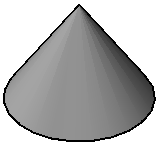
\includegraphics[scale=1]{yuanzhuiti.png}}\hspace{30pt}
\subfloat[]{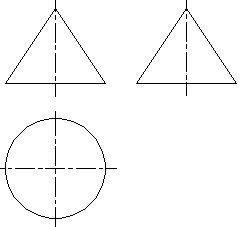
\includegraphics[scale=0.7]{yuanzhuitithreeview.png}}
\caption{圆锥体的投影}\label{fig:yuanzhuiti}
\end{figure}
\subsubsection{球体}
球体是由圆形母线以其直径为回转轴旋转而成的。球体的三面投影均为圆。
\begin{figure}[htbp]
\centering
\subfloat[]{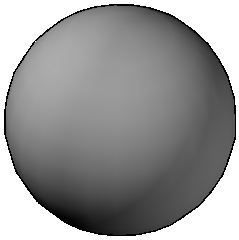
\includegraphics[scale=0.7]{qiouti.png}}\hspace{30pt}
\subfloat[]{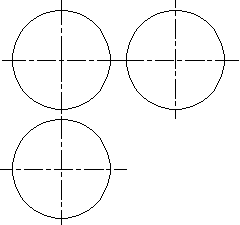
\includegraphics[scale=0.7]{qioutithreeview.png}}
\caption{球体的投影}\label{fig:qiout}
\end{figure}
\endinput
\section{法兰盘三视图}

{\bfseries 知识目标}
\begin{itemize}
\item 掌握回转体三视图规律
\end{itemize}

{\bfseries 技能目标}
\begin{itemize}
\item 能够应用三视图对应关系,运用AutoCAD绘制回转体的三视图
\end{itemize}

图\ref{fig:falanpanlititu}所示为工业中应用泛用于管道连接的法兰盘零件的简化形式。本任务主要是让读者了解并掌握回转体三视图表述方式,实现应用AutoCAD进行回转体类零件的三视图绘制的技能目标。
\begin{figure}[htbp]
\centering
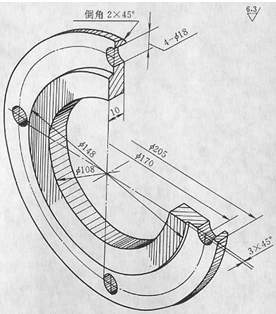
\includegraphics[scale=1]{fananlititu.png}
\caption{法兰盘}\label{fig:falanpanlititu}
\end{figure}
\subsection{绘制法兰盘主视图}
法兰盘整体是由两个圆筒叠加构成的,并具有四个用于安装的联接孔。我们先选择最能够表达的其形状的特征的方向作为其主视图。

具体绘图过程如下:

第一步:先定义图层,如图\ref{fig:falantucen}所示。
\begin{figure}[htbp]
\centering
\begin{floatrow}
\ffigbox{\caption{法兰盘图层定义}\label{fig:falantucen}}
{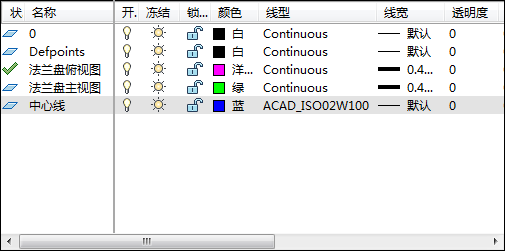
\includegraphics[scale=0.5]{falantucen.png}}
\ffigbox{\caption{法兰盘主视图}\label{fig:falanzhushitu}}{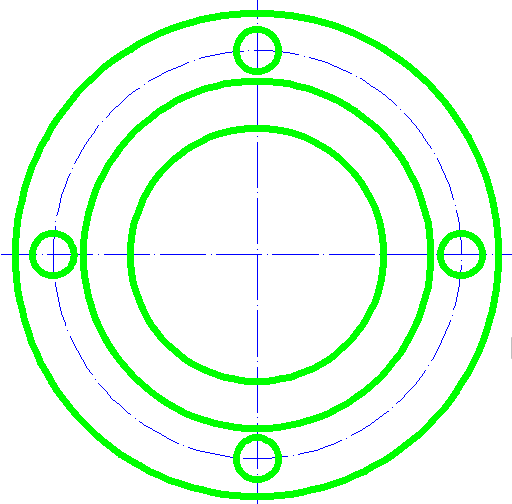
\includegraphics[scale=0.25]{falanzhushitu.png}}
\end{floatrow}
\end{figure}

第二步:绘制中心线,并完成主视图,如图\ref{fig:falanzhushitu}所示。

\begin{lstlisting}
%命令: line 指定第一点:%
%指定下一点或 [放弃(U)]: $@212<0$%
%指定下一点或 [放弃(U)]:%
%命令: LINE%
%指定第一点: @-106,106%
%指定下一点或 [放弃(U)]:$ @212<-90$%
%指定下一点或 [放弃(U)]:%
%命令: circle% 
%指定圆的圆心或 [三点(3P)/两点(2P)/切点、切点、半径(T)]: int%
%于%
%指定圆的半径或 [直径(D)]: 103%
%命令: circle %
%指定圆的圆心或 [三点(3P)/两点(2P)/切点、切点、半径(T)]: int%
%于%
%指定圆的半径或 [直径(D)]:$ <103.0000>$: 87%
%指定圆的圆心或 [三点(3P)/两点(2P)/切点、切点、半径(T)]: int%
%于%
%指定圆的半径或 [直径(D)]:$ <87.0000>$: 74%
%指定圆的圆心或 [三点(3P)/两点(2P)/切点、切点、半径(T)]: int%
%于%
%指定圆的半径或 [直径(D)]:$ <74.0000>$: 54%
%指定圆的圆心或 [三点(3P)/两点(2P)/切点、切点、半径(T)]: int%
%于%
%指定圆的半径或 [直径(D)]:$ <54.0000>$: 9%
%命令: arraypolar%
%选择对象: 找到 1 个%
%选择对象:%
%类型 = 极轴  关联 = 是%
%指定阵列的中心点或 [基点(B)/旋转轴(A)]: int%
%于%
%输入项目数或 [项目间角度(A)/表达式(E)]$ <4>:$%
%指定填充角度(+=逆时针、-=顺时针)或 [表达式(EX)] $<360>$:%
%按 Enter 键接受或 [关联(AS)/基点(B)/项目(I)/项目间角度(A)/填充%
%角度(F)/行(ROW)/层(L)/旋转项目(ROT)/退出(X)] %
%$<$退出$>$:%
\end{lstlisting}
\subsection{绘制法兰盘俯视图}
第一步:先利用长对正关系,确定定俯视图中对应部件的投影关系。
\begin{lstlisting}
%命令: line 指定第一点:%
%指定下一点或 [放弃(U)]: $ <$正交 开$>$%
%指定下一点或 [放弃(U)]:%
%命令: offset%
%当前设置: 删除源=否  图层=源  OFFSETGAPTYPE=0%
%指定偏移距离或 [通过(T)/删除(E)/图层(L)] %<%通过%>%:  10%
%选择要偏移的对象,或 [退出(E)/放弃(U)] $<$退出$>$:%
%指定要偏移的那一侧上的点,或 [退出(E)/多个(M)/放弃(U)] $<$退出$>$:%
%选择要偏移的对象,或 [退出(E)/放弃(U)] $<$退出$>$:%
%指定要偏移的那一侧上的点,或 [退出(E)/多个(M)/放弃(U)] $<$退出$>$:%
%选择要偏移的对象,或 [退出(E)/放弃(U)] $<$退出$>$:%
%命令: line %
%指定第一点: int%
%于%
%指定下一点或 [放弃(U)]: per%
%到%
%指定下一点或 [放弃(U)]:%
%命令: line %
%指定第一点: int%
%于%
%指定下一点或 [放弃(U)]: per%
%到%
%指定下一点或 [放弃(U)]:%
%命令: line %
%指定第一点: int%
%于%
%指定下一点或 [放弃(U)]: per%
%到%
%指定下一点或 [放弃(U)]:%
%命令: line %
%指定第一点: int%
%于%
%指定下一点或 [放弃(U)]: per%
%到%
%指定下一点或 [放弃(U)]:%
%命令: line %
%指定第一点: int%
%于%
%指定下一点或 [放弃(U)]: per%
%到%
%指定下一点或 [放弃(U)]:%
%命令: line %
%指定第一点: int%
%于%
%指定下一点或 [放弃(U)]: per%
%到%
%指定下一点或 [放弃(U)]:%
%命令: line %
%指定第一点: int%
%于%
%指定下一点或 [放弃(U)]: per%
%到%
%指定下一点或 [放弃(U)]:%
%命令: line %
%指定第一点: int%
%于%
%指定下一点或 [放弃(U)]: per%
%到%
%指定下一点或 [放弃(U)]:%
%命令: line %
%指定第一点: int%
%于%
%指定下一点或 [放弃(U)]: per%
%到%
%指定下一点或 [放弃(U)]:%
%命令: line %
%指定第一点: int%
%于%
%指定下一点或 [放弃(U)]: per%
%到%
%指定下一点或 [放弃(U)]:%
%命令: line %
%指定第一点: int%
%于%
%指定下一点或 [放弃(U)]: per%
%到%
%指定下一点或 [放弃(U)]:%
%命令: line %
%指定第一点: int%
%于%
%指定下一点或 [放弃(U)]: per%
%到%
%指定下一点或 [放弃(U)]:%
\end{lstlisting}

\begin{figure}[htbp]
\centering
\begin{floatrow}
\ffigbox{\caption{法兰盘俯视图}\label{fig:falanfushitu}}{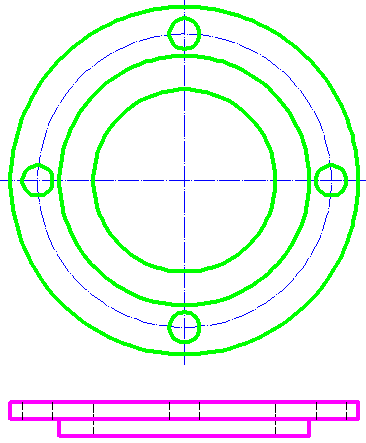
\includegraphics[scale=0.3]{falanfushitu.png}}
\ffigbox{\caption{法兰盘三视图}\label{fig:falansanshitu}}{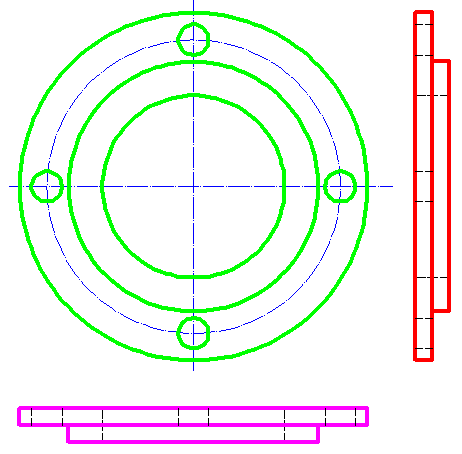
\includegraphics[scale=0.3]{falansanshitu.png}}
\end{floatrow}
\end{figure}

第二步:根据\ref{fig:falanpanlititu}所示尺寸绘出俯视图,如图\ref{fig:falanfushitu}所示。
\begin{lstlisting}
%命令: trim%
%当前设置:投影=UCS,边=无%
%选择剪切边...%
%选择对象或 $<$全部选择$>$:  找到 1 个%
%选择对象:%
%选择要修剪的对象,或按住 Shift 键选择要延伸的对象,或%
%[栏选(F)/窗交(C)/投影(P)/边(E)/删除(R)/放弃(U)]:  指定对角点:%
%选择要修剪的对象,或按住 Shift 键选择要延伸的对象,或%
%[栏选(F)/窗交(C)/投影(P)/边(E)/删除(R)/放弃(U)]:%
%命令: trim%
%当前设置:投影=UCS,边=无%
%选择剪切边...%
%选择对象或 $<$全部选择$>$:  找到 1 个%
%选择对象: 找到 1 个,总计 2 个%
%选择对象: 找到 1 个,总计 3 个%
%选择对象: 找到 1 个,总计 4 个%
%选择对象:%
%选择要修剪的对象,或按住 Shift 键选择要延伸的对象,或%
%[栏选(F)/窗交(C)/投影(P)/边(E)/删除(R)/放弃(U)]:  指定对角点:%
%选择要修剪的对象,或按住 Shift 键选择要延伸的对象,或%
%[栏选(F)/窗交(C)/投影(P)/边(E)/删除(R)/放弃(U)]:  指定对角点:%
%选择要修剪的对象,或按住 Shift 键选择要延伸的对象,或%
%[栏选(F)/窗交(C)/投影(P)/边(E)/删除(R)/放弃(U)]:%
%命令: TRIM%
%当前设置:投影=UCS,边=无%
%选择剪切边...%
%选择对象或 $<$全部选择$>$:  找到 1 个%
%选择对象:%
%选择要修剪的对象,或按住 Shift 键选择要延伸的对象,或%
%[栏选(F)/窗交(C)/投影(P)/边(E)/删除(R)/放弃(U)]:%
%选择要修剪的对象,或按住 Shift 键选择要延伸的对象,或%
%[栏选(F)/窗交(C)/投影(P)/边(E)/删除(R)/放弃(U)]:%
%选择要修剪的对象,或按住 Shift 键选择要延伸的对象,或%
%[栏选(F)/窗交(C)/投影(P)/边(E)/删除(R)/放弃(U)]:%
\end{lstlisting}

\subsection{绘制法兰盘左视图}
利用主、左高平齐,俯左宽相等的对应关系绘制左视图的相关部分,最终形成三视图如图\ref{fig:falansanshitu}所示。
\begin{lstlisting}
%命令: line 指定第一点:%
%指定下一点或 [放弃(U)]: $ <$正交 开$>$%
%指定下一点或 [放弃(U)]:%
%命令: offset%
%当前设置: 删除源=否  图层=源  OFFSETGAPTYPE=0%
%指定偏移距离或 [通过(T)/删除(E)/图层(L)] $<10.0000>$:  int%
%于  指定第二点: int%
%于%
%选择要偏移的对象,或 [退出(E)/放弃(U)] $<$退出$>$:%
%指定要偏移的那一侧上的点,或 [退出(E)/多个(M)/放弃(U)] $<$退出$>$:%
%选择要偏移的对象,或 [退出(E)/放弃(U)] $<$退出$>$:%
%命令: offset%
%当前设置: 删除源=否  图层=源  OFFSETGAPTYPE=0%
%指定偏移距离或 [通过(T)/删除(E)/图层(L)]$ <10.0000>$:  int%
%于  指定第二点: int%
%于%
%选择要偏移的对象,或 [退出(E)/放弃(U)] $<$退出$>$:%
%指定要偏移的那一侧上的点,或 [退出(E)/多个(M)/放弃(U)] $<$退出$>$:%
%选择要偏移的对象,或 [退出(E)/放弃(U)] $<$退出$>$:%
%命令: line %
%指定第一点: int%
%于%
%指定下一点或 [放弃(U)]: per%
%到%
%指定下一点或 [放弃(U)]:%
%命令: line %
%指定第一点: int%
%于%
%指定下一点或 [放弃(U)]: per%
%到%
%指定下一点或 [放弃(U)]:%
%命令: line %
%指定第一点: int%
%于%
%指定下一点或 [放弃(U)]: per%
%到%
%指定下一点或 [放弃(U)]:%
%命令: line %
%指定第一点: int%
%于%
%指定下一点或 [放弃(U)]: per%
%到%
%指定下一点或 [放弃(U)]:%
%命令: line %
%指定第一点: int%
%于%
%指定下一点或 [放弃(U)]: per%
%到%
%指定下一点或 [放弃(U)]:%
%命令: line %
%指定第一点: int%
%于%
%指定下一点或 [放弃(U)]: per%
%到%
%指定下一点或 [放弃(U)]:%
%命令: line %
%指定第一点: int%
%于%
%指定下一点或 [放弃(U)]: per%
%到%
%指定下一点或 [放弃(U)]:%
%命令: line %
%指定第一点: int%
%于%
%指定下一点或 [放弃(U)]: per%
%到%
%指定下一点或 [放弃(U)]:%
%命令: line %
%指定第一点: int%
%于%
%指定下一点或 [放弃(U)]: per%
%到%
%指定下一点或 [放弃(U)]:%
%命令: line %
%指定第一点: int%
%于%
%指定下一点或 [放弃(U)]: per%
%到%
%指定下一点或 [放弃(U)]:%
%命令: line %
%指定第一点: int%
%于%
%指定下一点或 [放弃(U)]: per%
%到%
%指定下一点或 [放弃(U)]:%
%命令: line %
%指定第一点: int%
%于%
%指定下一点或 [放弃(U)]: per%
%到%
%指定下一点或 [放弃(U)]:%
%命令: trim%
%当前设置:投影=UCS,边=无%
%选择剪切边...%
%选择对象或 $<$全部选择$>$:  找到 1 个%
%选择对象:%
%选择要修剪的对象,或按住 Shift 键选择要延伸的对象,或%
%[栏选(F)/窗交(C)/投影(P)/边(E)/删除(R)/放弃(U)]:  指定对角点:%
%选择要修剪的对象,或按住 Shift 键选择要延伸的对象,或%
%[栏选(F)/窗交(C)/投影(P)/边(E)/删除(R)/放弃(U)]:%
%命令: trim%
%当前设置:投影=UCS,边=无%
%选择剪切边...%
%选择对象或 $<$全部选择$>$:  找到 1 个%
%选择对象: 找到 1 个,总计 2 个%
%选择对象: 找到 1 个,总计 3 个%
%选择对象: 找到 1 个,总计 4 个%
%选择对象:%
%选择要修剪的对象,或按住 Shift 键选择要延伸的对象,或%
%[栏选(F)/窗交(C)/投影(P)/边(E)/删除(R)/放弃(U)]:  指定对角点:%
%选择要修剪的对象,或按住 Shift 键选择要延伸的对象,或%
%[栏选(F)/窗交(C)/投影(P)/边(E)/删除(R)/放弃(U)]:  指定对角点:%
%选择要修剪的对象,或按住 Shift 键选择要延伸的对象,或%
%[栏选(F)/窗交(C)/投影(P)/边(E)/删除(R)/放弃(U)]:%
%命令: TRIM%
%当前设置:投影=UCS,边=无%
%选择剪切边...%
%选择对象或 $<$全部选择$>$:  找到 1 个%
%选择对象:%
%选择要修剪的对象,或按住 Shift 键选择要延伸的对象,或%
%[栏选(F)/窗交(C)/投影(P)/边(E)/删除(R)/放弃(U)]:%
%选择要修剪的对象,或按住 Shift 键选择要延伸的对象,或%
%[栏选(F)/窗交(C)/投影(P)/边(E)/删除(R)/放弃(U)]:%
%选择要修剪的对象,或按住 Shift 键选择要延伸的对象,或%
%[栏选(F)/窗交(C)/投影(P)/边(E)/删除(R)/放弃(U)]:%
\end{lstlisting}
\endinput
\section{轴承支座三视图}

\endinput
\section{生成阀盖三视图}
\begin{procedure}
\item 打开“调压阀阀盖立体图.dwg”文件,并另存为“调压阀阀盖布局图.dwg”。

这样做的目的是为了保护源文件,以防止误操作后可进行有效的恢复之前的工作。AutoCAD本身并没有要求这样做。
\item 新建布局。

新建布局的方法有:
\begin{itemize}
\item 键盘输入LAYEROUT命令中的【新建N】选项。
\item 点击【插入】菜单中【布局】子菜单中的【新建布局】项。
\item 点击【插入】菜单中【布局】子菜单中的【创建布局向导】项。
\item 右击【模型】和【布局】
\includegraphics[scale=0.8]{buju.png} 区域,在弹出菜单中选择【新建布局】项。
\item 单击【模型】和【布局】
\includegraphics[scale=0.8]{buju.png} 区域中的【布局1】或【布局2】选项卡。
\item 点击【布局】工具栏中的【新建布局图标】
\includegraphics[scale=0.7]{buju1.png}
\end{itemize}
在此我们以【创建布向导】的方式来讲述如何新建布局。启动【创建布局】向导后会弹出图\ref{fig:bujuxiangdao1}所示对话框。
\begin{figure}[htbp]
\centering
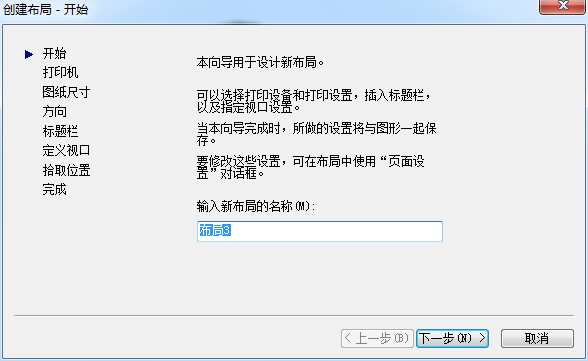
\includegraphics[scale=0.8]{bujuxiangdao1.png}
\caption{创建布局-开始对话框}\label{fig:bujuxiangdao1}
\end{figure}

此时,输入布局的名称并单下一步,弹出图\ref{fig:bujuxiangdao2}所示打印机设置对话框,将打印机设置为“DWG TO PDF.pc3"。实际工作中则就设置为可用的打印设备。
\begin{figure}[htbp]
\centering
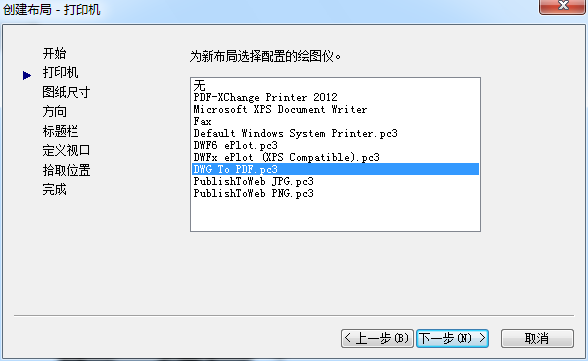
\includegraphics[scale=0.7]{bujuxiangdao2.png}
\caption{创建布局-打印机}\label{fig:bujuxiangdao2}
\end{figure}

设置完打印机后,单击下一步,弹出图\ref{fig:bujuxiangdao3}所示的图纸尺寸设置对话框。单击下拉框,将图纸设置为“ISO A4(297.00x210.00毫米)”,图形单位设置为毫米。
\begin{figure}[htbp]
\centering
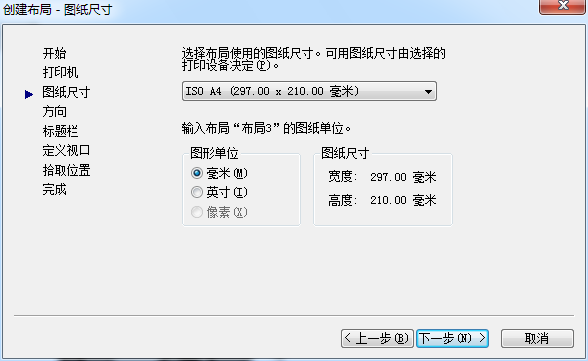
\includegraphics[scale=0.7]{bujuxiangdao3.png}
\caption{创建布局-图纸尺寸}\label{fig:bujuxiangdao3}
\end{figure}

设置完成后,单击下一步,弹出图\ref{fig:bujuxiangdao4}所示的方向设置对话框。此时将图形在图纸上的方向设置为横向。
\newpage
\begin{figure}[htbp]
\centering
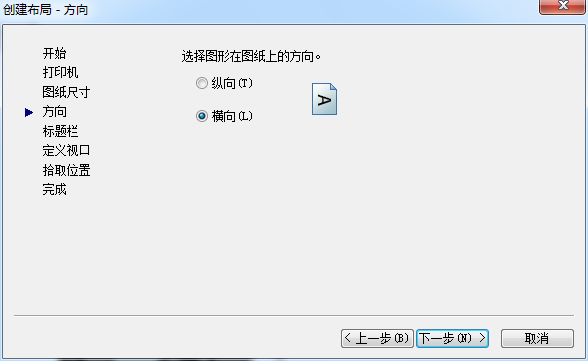
\includegraphics[scale=0.7]{bujuxiangdao4.png}
\caption{创建布局-方向}\label{fig:bujuxiangdao4}
\end{figure}

设置完成后,单击下一步,弹出图\ref{fig:bujuxiangdao5}所示的标题栏设置对话框。此时,将标题栏路径设置为无。
\begin{figure}[htbp]
\centering
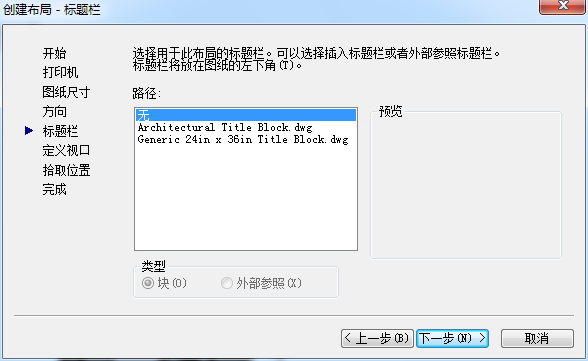
\includegraphics[scale=0.7]{bujuxiangdao5.png}
\caption{创建布局-标题栏}\label{fig:bujuxiangdao5}
\end{figure}

设置完成后,单击下一步,弹出图\ref{fig:bujuxiangdao6}所示的定义视口对话框。视口设置中单个表示创建一个视口,标准三维工程视图创建四个相等三个视口,阵列用于创建指定行和列的视口中。视口比例用于设置视口中显示对象的比例。由于生成三视图不需要用视口,因此在视口设置中选择无。
\newpage
\begin{figure}[htbp]
\centering
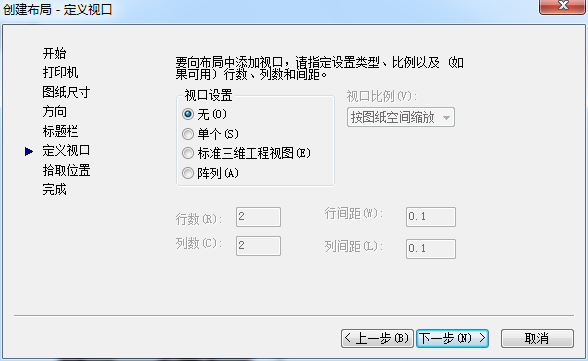
\includegraphics[scale=0.7]{bujuxiangdao6.png}
\caption{创建布局-定义视口}\label{fig:bujuxiangdao6}
\end{figure}

设置完成后,单击下一步,并点击完成,结束布局创建。
\item 从布局空间切换至模型空间。
\item 将工作空间由AutoCAD经典切换为三维建模,如图\ref{fig:sanweijianmo}所示。
\begin{figure}[htbp]
\centering
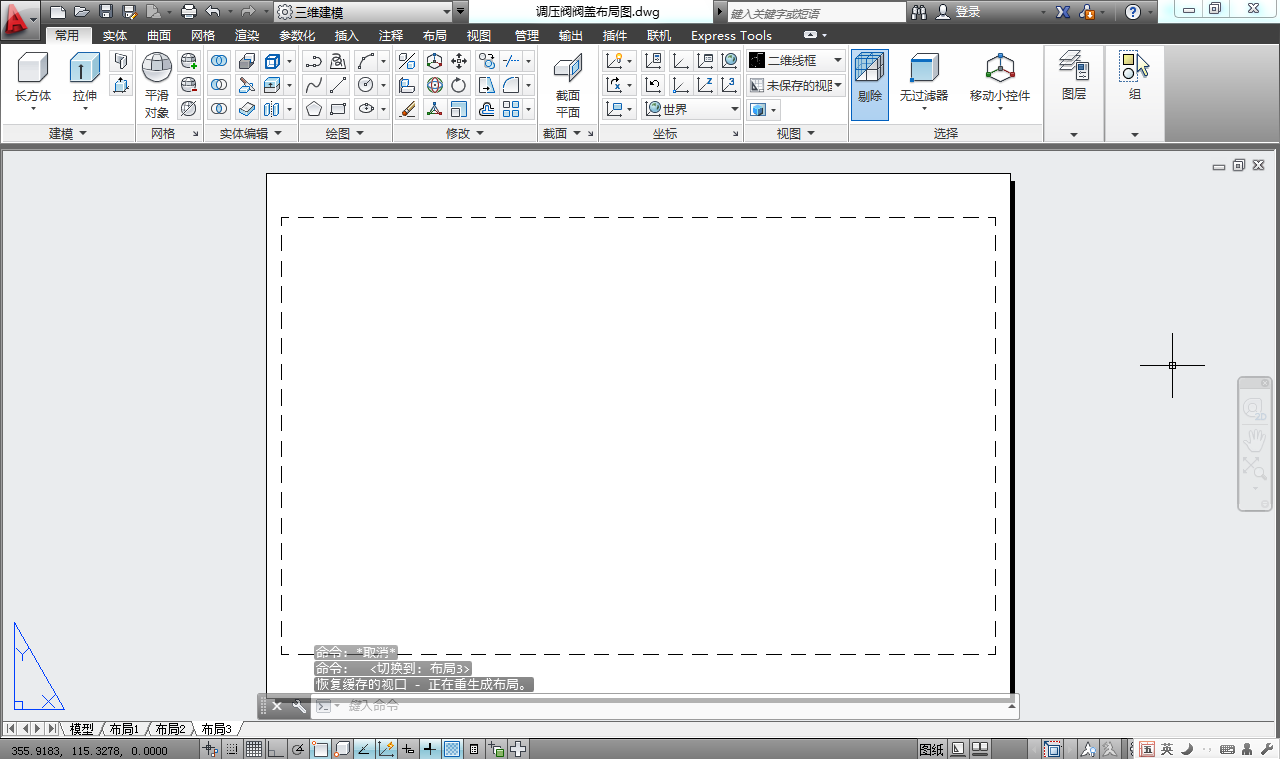
\includegraphics[scale=0.3]{sanweijianmo.png}
\caption{创建布局-定义视口}\label{fig:sanweijianmo}
\end{figure}
\item 创建基础视图。
启动创建基础视图的方法有:
\begin{itemize}
\item 键盘输出VIEWBASE。
\item 点【布局选项卡】中的【基础】图标
\includegraphics[scale=0.5]{viewbase.png},从下拉框中的选择
\includegraphics[scale=0.45]{comefrommodel.png}项
\end{itemize}
\newpage
启动命令后,选择从模式空间生成。
\begin{lstlisting}
|命令: VIEWBASE|
|指定模型源 [模型空间(M)/文件(F)] $<$模型空间$>$:
\end{lstlisting}
从模型空间中选择阀盖实体。
\begin{lstlisting}
|选择对象或 [整个模型(E)] $<$整个模型$>$: 找到 1 个|
|选择对象或 [整个模型(E)] $<$整个模型$>$:|
\end{lstlisting}
选择新创建的布局3作为生成的图纸。
\begin{lstlisting}
|输入要置为当前的新的或现有布局名称或 [?] $<$布局3$>$:|
|恢复缓存的视口 - 正在重生成布局。|
|命令:|
|类型 = 基础和投影  隐藏线 = 可见线和隐藏线  比例 = 1:1|
\end{lstlisting}
指定主视图的位置,如图\ref{fig:fagaibaseview1}所示。
\begin{lstlisting}
|指定基础视图的位置或 [类型(T)/选择(E)/方向(O)/隐藏线(H)/|
|比例(S)/可见性(V)] $<$类型$>$:|
|选择选项 [选择(E)/方向(O)/隐藏线(H)/比例(S)/可见性(V)/移动(M)|
|/退出(X)] $<$退出$>$:|
\end{lstlisting}
\begin{figure}[htbp]
\centering
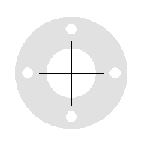
\includegraphics[scale=1.4]{fagaibaseview1.png}
\caption{指定主视图位置}\label{fig:fagaibaseview1}
\end{figure}
选择左视图的投影视图位置
\begin{lstlisting}
|指定投影视图的位置或 $<$退出$>$:|
\end{lstlisting}
\begin{figure}[htbp]
\centering
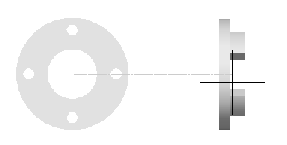
\includegraphics[scale=1.4]{fagaibaseview2.png}
\caption{指定左视图位置}\label{fig:fagaibaseview2}
\end{figure}
\newpage
选择俯视图的投影视图位置
\begin{lstlisting}
|指定投影视图的位置或 [放弃(U)/退出(X)] $<$退出$>$:|
|指定投影视图的位置或 [放弃(U)/退出(X)] $<$退出$>$:|
\end{lstlisting}
\begin{figure}[htbp]
\centering
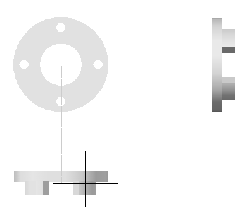
\includegraphics[scale=1.2]{fagaibaseview3.png}
\caption{指定左视图位置}\label{fig:fagaibaseview3}
\end{figure}
最终结果如图\ref{fig:fagaibaseview4} 所示。
\begin{figure}[htbp]
\centering
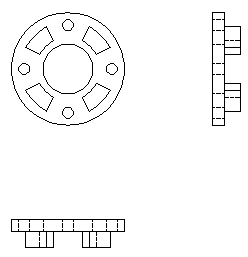
\includegraphics[scale=1.2]{fagaibaseview4.png}
\caption{阀盖三视图}\label{fig:fagaibaseview4}
\end{figure}
\end{procedure}
\endinput
\endinput